\PassOptionsToClass{12pt}{ccg-topic}
\documentclass{ccg-topic}
\topic{Probability in-depth}
\input{../repos/openintro-statistics/extraTeX/style/style.tex}
\input{../repos/openintro-statistics/extraTeX/style/colorsV1.tex}
\institution{University of Colorado}
\coursenum{MATH 2510-001}
\coursename{Introduction to Statistics}
\semester{Fall 2019}
\author{Diez, \c{C}etinkaya-Rundel, Barr (edited by Colton)}
\date{\today}
\email{colton.grainger@colorado.edu}
\thanks{These notes are scraped from the ``Probability" chapter of OpenIntro Statistics v4.0.}
\usepackage{graphicx, color}

\begin{document}
\setcounter{section}{1}
% \newcommand{\resp}[1]{\texttt{#1}} 
% \newcommand{\us}[1]{\textunderscore} 
% \newcommand{\data}[1]{\texttt{#1}}
\newcommand{\answer}[1]{\color{blue}#1}
\renewcommand{\chapterfolder}{ch_probability}
% \renewcommand{\var}[1]{\texttt{#1}}

%To display answers, replace "white" with "red" here;

\frontstuff
\begin{figure}[htpb]
    \centering
    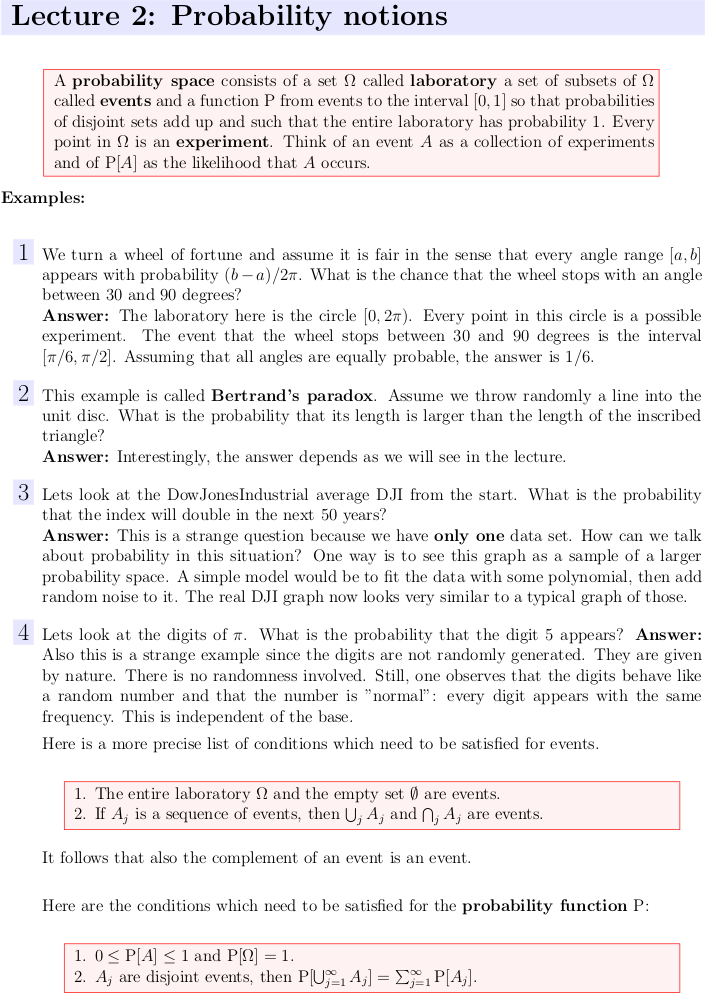
\includegraphics[width=0.57\linewidth]{2019-09-17-probability-notions.png}
    \caption{2011 Lecture notes from my hero, Oliver Knill.}
    \label{fig:2019-09-17-probability-notions}
\end{figure}
\printindex

\vspace{1em}\noindent\textsc{What's this next section all about?} \kw{Introductory examples}
\vspace{1em}

Before we get into technical ideas, let's walk through
some basic examples that may feel more familiar.

\begin{ex}{A ``die'', the singular of dice, is a cube with six faces numbered \resp{1}, \resp{2}, \resp{3}, \resp{4}, \resp{5}, and \resp{6}. What is the chance of getting \resp{1} when rolling a die?}\label{probOf1}
If the die is fair, then the chance of a \resp{1} is as good as the chance of any other number. Since there are six outcomes, the chance must be \ask{1-in-6} or, equivalently, \ask{$1/6$}.
\end{ex}

\begin{ex}{What is the chance of getting a \resp{1} or \resp{2} in the next roll?}\label{probOf1Or2}
\resp{1} and \resp{2} constitute two of the six equally likely possible outcomes, so the chance of getting one of these two outcomes must be \ask{$2/6 = 1/3$}.
\end{ex}

\begin{ex}{What is the chance of getting either \resp{1}, \resp{2}, \resp{3}, \resp{4}, \resp{5}, or \resp{6} on the next roll?}\label{probOf123456}
100\%. The outcome must be one of these numbers.
\end{ex}

\begin{ex}{What is the chance of not rolling a \resp{2}?}\label{probNot2}
Since the chance of rolling a \resp{2} is $1/6$ or $16.\bar{6}\%$, the chance of not rolling a \resp{2} must be $100\% - 16.\bar{6}\%=83.\bar{3}\%$ or $5/6$.

Alternatively, we could have noticed that not rolling a \resp{2} is the same as getting a \resp{1}, \resp{3}, \resp{4}, \resp{5}, or \resp{6}, which makes up five of the six equally likely outcomes and has probability $5/6$.
\end{ex}

\begin{ex}{Consider rolling two dice. If $1/6$ of the time the first die is a \resp{1} and $1/6$ of those times the second die is a \resp{1}, what is the chance of getting two \resp{1}s?}\label{probOf2Ones}
If $16.\bar{6}$\% of the time the first die is a \resp{1} and $1/6$ of \emph{those} times the second die is also a \resp{1}, then the chance that both dice are \resp{1} is $(1/6)\times (1/6)$ or $1/36$.
\end{ex}



\vspace{1em}\noindent\textsc{What's this next section all about?} \kw{Probability}
\vspace{1em}


We use probability to build tools to describe and understand apparent randomness. We often frame probability in terms of a \term{random process} giving rise to an \term{outcome}.
\begin{center}
\begin{tabular}{lll}
Roll a die &$\rightarrow$ & \resp{1}, \resp{2}, \resp{3}, \resp{4}, \resp{5}, or \resp{6} \\
Flip a coin &$\rightarrow$ & \resp{H} or \resp{T} \\
\end{tabular}
\end{center}
Rolling a die or flipping a coin is a seemingly random process and each gives rise to an outcome. 

\begin{defn}[Probability]
    The \term{probability} of an outcome is the proportion of times the outcome would occur if we observed the random process \ask{an infinite number} of times.
\end{defn}

Probability is defined as a proportion, and it always takes values between \ask{0~and~1} (inclusively). It may also be displayed as a percentage between 0\% and 100\%.

Probability can be illustrated by rolling a die many times. Let $\hat{p}_n$ be the proportion of outcomes that are \resp{1} after the first $n$ rolls. As the number of rolls increases, $\hat{p}_n$ will \ask{converge} to the probability of rolling a \resp{1}, $p = 1/6$. Figure~\ref{dieProp} shows this convergence for 100,000 die rolls. The tendency of $\hat{p}_n$ to stabilize around $p$ is described by the \kw{Law of Large Numbers}. 

\begin{figure}[h]
\centering
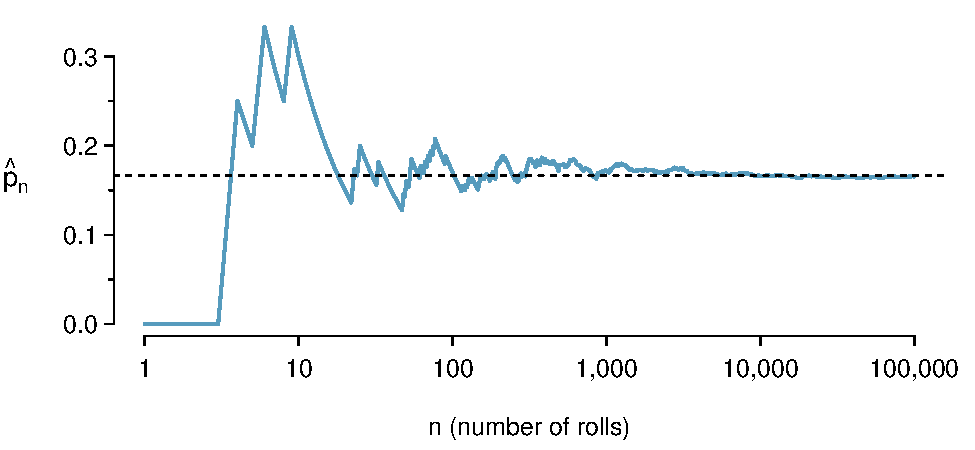
\includegraphics[width=0.85\textwidth]{ch_probability/figures/dieProp/dieProp}
\caption{The fraction of die rolls that are 1 at each stage in a simulation. The proportion tends to get closer to the probability $1/6 \approx 0.167$ as the number of rolls increases.}
\label{dieProp}
\end{figure}

\begin{defn}[Law of Large Numbers]
As more observations are collected, the proportion $\hat{p}_n$ of occurrences with a particular outcome \ask{converges to the probability} $p$ of that outcome.
\end{defn}

Occasionally the proportion will veer off from the probability and appear to defy the Law of Large Numbers, as $\hat{p}_n$ does many times in Figure~\ref{dieProp}. However, these deviations become smaller as the number of rolls increases.

Above we write $p$ as the probability of rolling a \resp{1}. We can also write this probability as \ask{$\P(\text{rolling a \resp{1}})$}. As we become more comfortable with this notation, we will abbreviate it further. For instance, if it is clear that the process is ``rolling a die'', we could abbreviate $\P(\text{rolling a 1})$ as \ask{$\P($\resp{1}$)$}. 

\begin{todo} \label{randomProcessExercise}
Random processes include rolling a die and flipping a coin. (a) Think of another random process. (b) Describe all the possible outcomes of that process. For instance, rolling a die is a random process with possible outcomes \mbox{\resp{1}, \resp{2}, ..., \resp{6}}.\footnotemark
\end{todo}
\footnotetext{Here are four examples. (i) Whether someone gets sick in the next month or not is an apparently random process with outcomes \resp{sick} and \resp{not}. (ii) We can \emph{generate} a random process by randomly picking a person and measuring that person's height. The outcome of this process will be a positive number. (iii) Whether the stock market goes up or down next week is a seemingly random process with possible outcomes \resp{up}, \resp{down}, and \resp{no\us{}change}. Alternatively, we could have used the percent change in the stock market as a numerical outcome. (iv) Whether your roommate cleans her dishes tonight probably seems like a random process with possible outcomes \resp{cleans\us{}dishes} and \resp{leaves\us{}dishes}.}

What we think of as random processes are not necessarily random, but they may just be too difficult to understand exactly. The fourth example in the footnote solution to Exercise~\ref{randomProcessExercise} suggests a roommate's behavior is a random process. However, even if a roommate's behavior is not truly random, modeling her behavior as a random process can still be useful. 

%\begin{tipBox}{\tipBoxTitle{Modeling a process as random}
%It can be helpful to model a process as random even if it is not truly random.}
%\end{tipBox}


\vspace{1em}\noindent\textsc{What's this next section all about?} \kw{Disjoint or mutually exclusive outcomes}

Two outcomes are called \kw{disjoint} or \kw{mutually exclusive} if they cannot both happen. For instance, if we roll a die, the outcomes \resp{1} and \resp{2} are disjoint since they cannot both occur. On the other hand, the outcomes \resp{1} and ``rolling an odd number'' are not disjoint since both occur if the outcome of the roll is a \resp{1}. The terms \emph{disjoint} and \emph{mutually exclusive} are equivalent and interchangeable.

Calculating the probability of disjoint outcomes is easy. When rolling a die, the outcomes \resp{1} and \resp{2} are disjoint, and we compute the probability that one of these outcomes will occur by \ask{adding} their \ask{separate} probabilities:
\begin{align*}
\P(\text{\resp{1} or \resp{2}})
  = \P(\text{\resp{1}})+\P(\text{\resp{2}})
  = 1/6 + 1/6
  = 1/3
\end{align*}
What about  the probability of rolling a \resp{1}, \resp{2}, \resp{3}, \resp{4}, \resp{5}, or \resp{6}? Here again, all of the outcomes are disjoint so we add the probabilities:
\begin{align*}
&\P(\text{\resp{1} or \resp{2} or \resp{3} or \resp{4}
    or \resp{5} or \resp{6}}) \\
  &\quad = \P(\text{\resp{1}})+\P(\text{\resp{2}})
      + \P(\text{\resp{3}})+\P(\text{\resp{4}})
      + \P(\text{\resp{5}})+\P(\text{\resp{6}}) \\
  &\quad = 1/6 + 1/6 + 1/6 + 1/6 + 1/6 + 1/6
  = 1
\end{align*}
The \term{Addition Rule} guarantees the accuracy of this approach when the outcomes are disjoint. 

\begin{defn}[Addition Rule of disjoint outcomes]
  If $A_1$ and $A_2$ represent two \kw{disjoint outcomes},
  then the probability that one of them occurs is given by
  \begin{center}
      \ask{$\P(A_1\text{ or } A_2) = \P(A_1) + \P(A_2)$}
  \end{center}
  If there are many disjoint outcomes $A_1$, ..., $A_k$,
  then the probability that one of these outcomes will occur is
  \begin{align*}
  \P(A_1) + \P(A_2) + \cdots + \P(A_k)
  \end{align*}
\end{defn}


\begin{todo}
We are interested in the probability of rolling a \resp{1}, \resp{4}, or \resp{5}. (a) Explain why the outcomes \resp{1}, \resp{4}, and \resp{5} are disjoint. (b) Apply the Addition Rule for disjoint outcomes to determine $P($\resp{1} or \resp{4} or \resp{5}$)$.\footnotemark
\end{todo}
\footnotetext{(a) The random process is a die roll, and at most one of these outcomes can come up. This means they are disjoint outcomes. (b)~$\P($\resp{1} or \resp{4} or \resp{5}$) = \P($\resp{1}$)+\P($\resp{4}$)+\P($\resp{5}$) = \frac{1}{6} + \frac{1}{6} + \frac{1}{6} = \frac{3}{6} = \frac{1}{2}$}

\begin{todo}
    In the \data{loans} data set in ``Summarizing Data'' (OpenIntro Statistics)
the \var{homeownership} variable described whether the borrower
rents, has a mortgage, or owns her property.
Of the 10,000 borrowers, 3858 rented, 4789 had a mortgage,
and 1353 owned their home.\footnotemark{}
\begin{enumerate}
\item Are the outcomes \resp{rent}, \resp{mortgage}, and \resp{own} disjoint?
\item Determine the proportion of loans with value \resp{mortgage} and \resp{own} separately.
\item Use the Addition Rule for disjoint outcomes to compute the probability a randomly selected loan from the data set is for someone who has a mortgage or owns her home.
\end{enumerate}
\end{todo}
\footnotetext{(a)~Yes. Each loan is categorized in only one
level of \var{homeownership}.
(b)~Mortgage: $\frac{4789}{10000} = 0.479$.
Own: $\frac{1353}{10000} = 0.135$.
(c)~$\P($\resp{mortgage} or \resp{own}$) = \P($\resp{mortgage}$) + \P($\resp{own}$) = 0.479 + 0.135 = 0.614$.}


Data scientists rarely work with individual outcomes and instead consider \kw{\emph{sets}} or \kw{\emph{collections}} of outcomes. Let $A$ represent the event where a die roll results in \resp{1} or \resp{2} and $B$~represent the event that the die roll is a \resp{4} or a \resp{6}. We write $A$ as the set of outcomes $\{$\resp{1},~\resp{2}$\}$ and $B=\{$\resp{4}, \resp{6}$\}$. These sets are commonly called \kw{events}. Because $A$ and $B$ have no elements in common, they are disjoint events. $A$ and $B$ are represented in Figure~\ref{disjointSets}.

\begin{figure}[hhh]
  \centering
  \Figure{0.45}{disjointSets}
  \caption{Three events, $A$, $B$, and $D$, consist of
      outcomes from rolling a die.
      $A$ and $B$ are disjoint since they do not have
      any outcomes in common.}
  \label{disjointSets}
\end{figure}

The Addition Rule applies to both disjoint outcomes and disjoint events. The probability that one of the disjoint events $A$ or $B$ occurs is the sum of the separate probabilities:
\begin{align*}
\P(A\text{ or }B) = \P(A) + \P(B) = 1/3 + 1/3 = 2/3
\end{align*}

\begin{todo}
(a) Verify the probability of event $A$, $P(A)$,
is $1/3$ using the Addition Rule.
(b)~Do the same for event $B$.\footnotemark
\end{todo}
\footnotetext{(a)~$\P(A) = \P($\resp{1} or \resp{2}$)
    = \P($\resp{1}$) + \P($\resp{2}$)
    = \frac{1}{6} + \frac{1}{6}
    = \frac{2}{6}
    = \frac{1}{3}$.
    (b)~Similarly, $\P(B) = 1/3$.}

\begin{todo} \label{exerExaminingDisjointSetsABD}
(a) Using Figure~\ref{disjointSets} as a reference, what outcomes are represented by event $D$? (b) Are events $B$ and $D$ disjoint? (c) Are events $A$ and $D$ disjoint?\footnotemark
\end{todo}
\footnotetext{(a)~Outcomes \resp{2} and \resp{3}. (b)~Yes, events $B$ and $D$ are disjoint because they share no outcomes. (c)~The events $A$ and $D$ share an outcome in common, \resp{2}, and so are not disjoint.}

\begin{todo}
In Exercise~\ref{exerExaminingDisjointSetsABD}, you confirmed $B$ and $D$ from Figure~\ref{disjointSets} are disjoint. Compute the probability that event $B$ or event $D$~occurs.\footnotemark
\end{todo}
\footnotetext{Since $B$ and $D$ are disjoint events, use the Addition Rule: $P(B$ or $D) = P(B) + P(D) = \frac{1}{3} + \frac{1}{3} = \frac{2}{3}$.}




\vspace{1em}\noindent\textsc{What's this next section all about?} \kw{Probabilities when events are not disjoint}
\vspace{1em}

Let's consider calculations for two events that are not disjoint in the context of a \kw{regular deck of 52 cards}, represented in Figure~\ref{deckOfCards}. If you are unfamiliar with the cards in a regular deck, please see the footnote.\footnote{The 52 cards are split into four \term{suits}: $\clubsuit$ (club), {\color{red}$\diamondsuit$} (diamond), {\color{red}$\heartsuit$} (heart), $\spadesuit$ (spade). Each suit has its 13 cards labeled: \resp{2}, \resp{3}, ..., \resp{10}, \resp{J} (jack), \resp{Q} (queen), \resp{K} (king), and \resp{A} (ace). Thus, each card is a unique combination of a suit and a label, e.g. {\color{red}\resp{4$\heartsuit$}} and \resp{J$\clubsuit$}. The 12 cards represented by the jacks, queens, and kings are called \kw{\resp{face cards}}. The cards that are {\color{red}$\diamondsuit$} or {\color{red}$\heartsuit$} are typically colored {\color{red}red} while the other two suits are typically colored black.}

\begin{figure}[h]
\centering
\begin{tabular}{lll lll lll lll l}
\resp{2$\clubsuit$} & \resp{3$\clubsuit$} & \resp{4$\clubsuit$} & \resp{5$\clubsuit$} & \resp{6$\clubsuit$} & \resp{7$\clubsuit$} & \resp{8$\clubsuit$} & \resp{9$\clubsuit$} & \resp{10$\clubsuit$} & \resp{J$\clubsuit$} & \resp{Q$\clubsuit$} & \resp{K$\clubsuit$} & \resp{A$\clubsuit$}  \\
\color{red} \resp{2$\diamondsuit$} & \color{red}\resp{3$\diamondsuit$} & \color{red}\resp{4$\diamondsuit$} & \color{red}\resp{5$\diamondsuit$} & \color{red}\resp{6$\diamondsuit$} & \color{red}\resp{7$\diamondsuit$} & \color{red}\resp{8$\diamondsuit$} & \color{red}\resp{9$\diamondsuit$} & \color{red}\resp{10$\diamondsuit$} & \color{red}\resp{J$\diamondsuit$} & \color{red}\resp{Q$\diamondsuit$} & \color{red}\resp{K$\diamondsuit$} & \color{red}\resp{A$\diamondsuit$} \\
\color{red}\resp{2$\heartsuit$} & \color{red}\resp{3$\heartsuit$} & \color{red}\resp{4$\heartsuit$} & \color{red}\resp{5$\heartsuit$} & \color{red}\resp{6$\heartsuit$} & \color{red}\resp{7$\heartsuit$} & \color{red}\resp{8$\heartsuit$} & \color{red}\resp{9$\heartsuit$} & \color{red}\resp{10$\heartsuit$} & \color{red}\resp{J$\heartsuit$} & \color{red}\resp{Q$\heartsuit$} & \color{red}\resp{K$\heartsuit$} & \color{red}\resp{A$\heartsuit$} \\
\resp{2$\spadesuit$} & \resp{3$\spadesuit$} & \resp{4$\spadesuit$} & \resp{5$\spadesuit$} & \resp{6$\spadesuit$} & \resp{7$\spadesuit$} & \resp{8$\spadesuit$} & \resp{9$\spadesuit$} & \resp{10$\spadesuit$} & \resp{J$\spadesuit$} & \resp{Q$\spadesuit$} & \resp{K$\spadesuit$} & \resp{A$\spadesuit$}
\end{tabular}
\caption{Representations of the 52 unique cards in a deck.}
\label{deckOfCards}
\end{figure}

\begin{todo}
(a) What is the probability that a randomly selected card is a diamond? (b)~What is the probability that a randomly selected card is a face card?\footnotemark
\end{todo}
\footnotetext{(a) There are 52 cards and 13 diamonds. If the cards are thoroughly shuffled, each card has an equal chance of being drawn, so the probability that a randomly selected card is a diamond is $P({\color{red}\diamondsuit}) = \frac{13}{52} = 0.250$. (b)~Likewise, there are 12 face cards, so $P($face card$) = \frac{12}{52} = \frac{3}{13} = 0.231$.}

\kw{Venn diagrams} are useful when outcomes can be categorized as ``in'' or ``out'' for two or three variables, attributes, or random processes. The Venn diagram in Figure~\ref{cardsDiamondFaceVenn} uses a circle to represent diamonds and another to represent face cards. If a card is both a diamond and a face card, it falls into the \ask{intersection} of the circles. If it is a diamond but not a face card, it will be in part of the \ask{left circle} that is not in the \ask{right circle} (and so on). The total number of cards that are diamonds is given by the total number of cards in the diamonds circle: $10+3=13$. The probabilities are also shown (e.g. $10/52 = 0.1923$).

\begin{figure}[h]
\centering
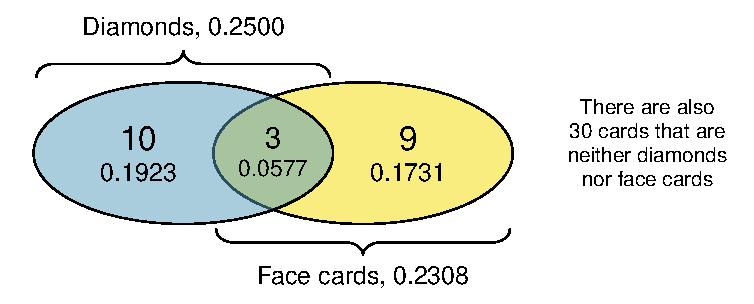
\includegraphics[width=0.65\textwidth]{ch_probability/figures/cardsDiamondFaceVenn/cardsDiamondFaceVenn}
\caption{A Venn diagram for diamonds and face cards.}
\label{cardsDiamondFaceVenn}
\end{figure}

Let $A$ represent the event that a randomly selected card is a diamond and $B$ represent the event that it is a face card. How do we compute $\P(A$ or $B)$? Events $A$ and $B$ are not disjoint -- the cards {\color{red}$J\diamondsuit$}, {\color{red}$Q\diamondsuit$}, and {\color{red}$K\diamondsuit$} fall into both categories -- so we cannot use the Addition Rule for disjoint events. Instead we use the Venn diagram. We start by \ask{adding the probabilities of the two events}:
\begin{align*}
\P(A) + \P(B)
  = \P({\color{red}\diamondsuit}) + \P(\text{face card})
  = 13/52 + 12/52
\end{align*}
\noindent However, the three cards that are in both events were \ask{counted twice}, once in each probability. We must correct this double counting:
\begin{align*}
\P(A\text{ or } B)
  &= \P({\color{red}\diamondsuit}\text{ or face card}) \\
  &= \P({\color{red}\diamondsuit}) + \P(\text{face card})
      - \P({\color{red}\diamondsuit}\text{ and face card}) \\
  &= 13/52 + 12/52 - 3/52 \\
  &= 22/52 = 11/26
\end{align*}
This equation is an example of the \term{General Addition Rule}. 

\begin{defn}
    \ask{General Addition Rule}
  If $A$ and $B$ are any two events, disjoint or not, then
  the probability that at least one of them will occur is
  \begin{center}
      $\P(A\text{ or }B) = \P(A) + \P(B) - $ \ask{$\P(A\text{ and }B)$}
  \end{center}
  where $\P(A$ and $B)$ is the probability that both events occur.
\end{defn}

\begin{tipBox}{\tipBoxTitle{``or'' is inclusive}
When we write ``or'' in statistics, we mean ``and/or'' unless we explicitly state otherwise. Thus, $A$ or $B$ occurs means $A$, $B$, or both $A$ and $B$ occur.}
\end{tipBox}

\begin{todo}
(a) If $A$ and $B$ are disjoint, describe why this implies $P(A$ and $B) = 0$. (b) Using part (a), verify that the General Addition Rule simplifies to the simpler Addition Rule for disjoint events if $A$ and $B$ are disjoint.\footnotemark
\end{todo}
\footnotetext{(a) If $A$ and $B$ are disjoint, $A$ and $B$ can never occur simultaneously. (b) If $A$ and $B$ are disjoint, then the last $\P(A\text{ and }B)$ term of in the General Addition Rule formula is 0 (see part (a)) and we are left with the Addition Rule for disjoint events.}


\begin{todo}\label{emailSpamNumberVennExer}
% library(openintro); d <- loans_full_schema; table(d[,c("application_type", "homeownership")]); table(d[,c("application_type")]); table(d[,c("homeownership")])
In the \data{loans} data set describing 10,000 loans,
1495 loans were from joint applications
(e.g. a couple applied together),
4789 applicants had a mortgage,
and 950 had both of these characteristics.
Create a Venn diagram for this setup.\footnotemark
\end{todo}
\footnotetext{%
  \begin{minipage}[t]{0.65\textwidth}
  Both the counts and corresponding {\color{blue}probabilities}
  (e.g. $3839/10000 = 0.384$) are shown.
  Notice that the number of loans represented in the left
  circle corresponds to $3839 + 950 = 4789$, and the number
  represented in the right circle is $950 + 545 = 1495$.
  \end{minipage}\ %
  \begin{minipage}[c]{0.3\textwidth}
  \hfill\Figure{1.00}{loans_app_type_home_venn} \vspace{-13mm}
  \end{minipage}}

\begin{todo}
(a)~Use your Venn diagram from Exercise~\ref{emailSpamNumberVennExer} to determine the
probability a randomly drawn loan from the \data{loans}
data set is from a joint application where the couple had
a mortgage.
(b)~What is the probability that the loan had either of
these attributes?\footnotemark
\end{todo}
\footnotetext{%
  (a)~The solution is represented by the intersection of
  the two circles: 0.095.
  (b)~This is the sum of the three disjoint probabilities shown
  in the circles: $0.384 + 0.095 + 0.055 = 0.534$
  (off by 0.001 due to a rounding error).}




\vspace{1em}\noindent\textsc{What's this next section all about?} \kw{Probability distributions}
\vspace{1em}

A \kw{probability distribution} is a table of all disjoint outcomes and their associated probabilities. Figure~\ref{diceProb} shows the probability distribution for the sum of two dice. 

\begin{figure}[h] \small
\centering
\begin{tabular}{l ccc ccc ccc cc}
  \hline
  \ \vspace{-3mm} \\
Dice sum\vspace{0.3mm} & 2 & 3 & 4 & 5 & 6 & 7 & 8 & 9 & 10 & 11 & 12  \\
Probability & $\frac{1}{36}$ & $\frac{2}{36}$ & $\frac{3}{36}$ & $\frac{4}{36}$ & $\frac{5}{36}$ & $\frac{6}{36}$ & $\frac{5}{36}$ & $\frac{4}{36}$ & $\frac{3}{36}$ & $\frac{2}{36}$ & $\frac{1}{36}$\vspace{1mm} \\
   \hline
\end{tabular}
\caption{Probability distribution for the sum of two dice.}
\label{diceProb}
\end{figure}

\begin{defn}{Rules for probability distributions}
A probability distribution is a list of the possible outcomes with corresponding probabilities that satisfies three rules: \vspace{-2mm}
\begin{enumerate}
\setlength{\itemsep}{0mm}
\item The outcomes listed must be disjoint.
\item Each probability must be between 0 and 1.
\item The probabilities must total 1. \vspace{1mm}
\end{enumerate}
\end{defn}

\begin{todo}\label{usHouseholdIncomeDistsExercise}
Figure~\ref{usHouseholdIncomeDists} suggests three distributions for household income in the United States. Only one is correct. Which one must it be? What is wrong with the other two?\footnotemark
\end{todo}
\footnotetext{The probabilities of (a) do not sum to~1.
    The second probability in (b) is negative.
    This leaves~(c), which sure enough satisfies the
    requirements of a distribution.
    One of the three was said to be the actual
    distribution of US household incomes,
    so it must be~(c).}

\begin{figure}[h]
\centering
\begin{tabular}{r | cc cc}
  \hline
Income Range & \$0-25k & \$25k-50k & \$50k-100k & \$100k+ \\
  \hline
(a)\hspace{0.2mm}	 & 0.18 & 0.39 & 0.33 & 0.16 \\
(b)				 & 0.38 & -0.27 & 0.52 & 0.37 \\
(c)\hspace{0.2mm}	 & 0.28 & 0.27 & 0.29 & 0.16 \\
  \hline
\end{tabular}
\caption{Proposed distributions of US household incomes (Exercise~\ref{usHouseholdIncomeDistsExercise}).}
\label{usHouseholdIncomeDists}
\end{figure}

The first three weeks of our course emphasized the importance of plotting data to provide quick summaries. Probability distributions can also be summarized in a bar plot. For instance, the distribution of US household incomes is shown in Figure~\ref{usHouseholdIncomeDistBar} as a bar plot. %\footnote{It is also possible to construct a distribution plot when income is not artificially binned into four groups. \emph{Continuous} distributions are considered in Section~\ref{contDist}.}
The probability distribution for the sum of two dice is shown in Figure~\ref{diceProb} and plotted in Figure~\ref{diceSumDist}.

\begin{figure}[h]
  \centering
  \Figure{0.65}{usHouseholdIncomeDistBar}
  \caption{The probability distribution of US household income.}
  \label{usHouseholdIncomeDistBar}
\end{figure}

\begin{figure}
  \centering
  \Figure{0.67}{diceSumDist}
  \caption{The probability distribution of the sum of two dice.}
  \label{diceSumDist}
\end{figure}

In these bar plots, the bar heights represent the probabilities of outcomes. If the outcomes are numerical and discrete, it is usually (visually) convenient to make a bar plot that resembles a histogram, as in the case of the sum of two dice. 

\vspace{1em}\noindent\textsc{What's this next section all about?} \kw{Complement of an event}
\vspace{1em}

Rolling a die produces a value in the set $\{$\resp{1}, \resp{2}, \resp{3}, \resp{4}, \resp{5}, \resp{6}$\}$. This set of all possible outcomes is called the \kw{sample space} (denoted by \kw{$S$ or $\Omega$}) for rolling a die. We often use the sample space to examine the scenario where an event does not occur.

Let $D=\{$\resp{2}, \resp{3}$\}$ represent the event that the outcome of a die roll is \resp{2} or \resp{3}. Then the \kw{complement} of $D$ represents all outcomes in our sample space that are not in $D$, which is denoted by $D^c = \{$\resp{1}, \resp{4}, \resp{5}, \resp{6}$\}$. That is, $D^c$ is the set of all possible outcomes not already included in $D$. Figure~\ref{complementOfD} shows the relationship between $D$, $D^c$, and the sample space $S$. 

\begin{figure}[hht]
  \centering
  \Figure{0.55}{complementOfD}
  \caption{Event $D=\{$\resp{2}, \resp{3}$\}$ and its complement,
      $D^c = \{$\resp{1}, \resp{4}, \resp{5}, \resp{6}$\}$.
      $S$~represents the sample space, which is the set of
      all possible outcomes.}
  \label{complementOfD}
\end{figure}

\begin{todo}
(a) Compute $\P(D^c) = \P($rolling a \resp{1}, \resp{4}, \resp{5}, or \resp{6}$)$. (b) What is $\P(D) + \P(D^c)$?\footnotemark
\end{todo}
\footnotetext{(a)~The outcomes are disjoint and each has probability $1/6$, so the total probability is $4/6=2/3$. (b)~We can also see that $\P(D)=\frac{1}{6} + \frac{1}{6} = 1/3$. Since $D$ and $D^c$ are disjoint, $\P(D) + \P(D^c) = 1$.}

\begin{todo}
Events $A=\{$\resp{1}, \resp{2}$\}$ and $B=\{$\resp{4}, \resp{6}$\}$ are shown in Figure~\ref{disjointSets} on page~\pageref{disjointSets}. (a) Write out what $A^c$ and $B^c$ represent. (b)~Compute $\P(A^c)$ and $\P(B^c)$. (c)~Compute $\P(A)+\P(A^c)$ and $\P(B)+\P(B^c)$.\footnotemark
\end{todo}
\footnotetext{Brief solutions: (a)~$A^c=\{$\resp{3}, \resp{4}, \resp{5}, \resp{6}$\}$ and $B^c=\{$\resp{1}, \resp{2}, \resp{3}, \resp{5}$\}$. (b)~Noting that each outcome is disjoint, add the individual outcome probabilities to get $\P(A^c)=2/3$ and $\P(B^c)=2/3$. (c)~$A$~and~$A^c$ are disjoint, and the same is true of $B$~and~$B^c$. Therefore, $\P(A) + \P(A^c) = 1$ and $\P(B) + \P(B^c) = 1$.}


A complement of an event $A$ is constructed to have two very important properties: (i) every possible outcome not in $A$ is in $A^c$, and (ii) $A$ and $A^c$ are disjoint. Property (i) implies
\begin{align*}
\P(A\text{ or }A^c) = 1
\end{align*}
That is, if the outcome is not in $A$, it must be represented in $A^c$. We use the Addition Rule for disjoint events to apply Property (ii):
\begin{align*}
\P(A\text{ or }A^c) = \P(A) + \P(A^c)
\end{align*}
Combining the last two equations yields a very useful
relationship between the probability of an event and
its complement.

\begin{defn}[Complement]
  The complement of event $A$ is denoted $A^c$, and $A^c$
  represents all outcomes not in~$A$. $A$ and $A^c$ are
  mathematically related:
  \begin{align*}
  \P(A) + \P(A^c) = 1, \quad\text{i.e.}\quad \P(A) = 1-\P(A^c)
  \end{align*}
\end{defn}

In simple examples, computing $A$ or $A^c$ is feasible in a few steps. However, using the complement can \ask{save a lot of time} as problems grow in complexity.

\begin{todo}
Let $A$ represent the event where we roll two dice and their total is less than \resp{12}. (a)~What does the event $A^c$ represent? (b)~Determine $\P(A^c)$ from Figure~\ref{diceProb} on page~\pageref{diceProb}. (c)~Determine $\P(A)$.\footnotemark
\end{todo}
\footnotetext{(a)~The complement of $A$: when the total is equal to \resp{12}. (b)~$\P(A^c) = 1/36$. (c)~Use the probability of the complement from part (b), $\P(A^c) = 1/36$, and the equation for the complement: $\P($less than \resp{12}$) = 1 - \P($\resp{12}$) = 1 - 1/36 = 35/36$.}

\begin{todo}
Find the following probabilities for rolling two dice:\footnotemark
\begin{enumerate}
\setlength{\itemsep}{0mm}
\item The sum of the dice is \emph{not} \resp{6}. 
\item The sum is at least \resp{4}.
    That is, determine the probability of the event
    $B = \{$\resp{4}, \resp{5}, ..., \resp{12}$\}$.
\item The sum is no more than \resp{10}.
    That is, determine the probability of the event
    $D=\{$\resp{2}, \resp{3}, ..., \resp{10}$\}$.
\end{enumerate}
\end{todo}
\footnotetext{(a)~First find $\P($\resp{6}$)=5/36$, then use the complement: $\P($not \resp{6}$) = 1 - \P($\resp{6}$) = 31/36$.

(b)~First find  the complement, which requires much less effort: $\P($\resp{2} or \resp{3}$)=1/36+2/36=1/12$. Then calculate $\P(B) = 1-\P(B^c) = 1-1/12 = 11/12$.

(c)~As before, finding the complement is the clever way to determine $\P(D)$. First find $\P(D^c) = \P($\resp{11} or \resp{12}$)=2/36 + 1/36=1/12$. Then calculate $\P(D) = 1 - \P(D^c) = 11/12$.}


\vspace{1em}\noindent\textsc{What's this next section all about?} \kw{Independence}
\vspace{1em}

Just as variables and observations can be independent, random processes can be independent, too. Two processes are \kw{independent} if knowing the outcome of one provides no useful information about the outcome of the other. For instance, flipping a coin and rolling a die are two \ask{independent processes (or events)} --- knowing the coin was heads does not help determine the outcome of a die roll. On the other hand, stock prices usually move up or down together, so they are not independent.

Example~\ref{probOf2Ones} provides a basic example of two independent processes: rolling two dice. We want to determine the probability that both will be \resp{1}. Suppose one of the dice is red and the other white. If the outcome of the red die is a \resp{1}, it provides no information about the outcome of the white die. We first encountered this same question in Example~\ref{probOf2Ones} (page~\pageref{probOf2Ones}), where we calculated the probability using the following reasoning: $1/6$ of the time the red die is a \resp{1}, and $1/6$ of \emph{those} times the white die will also be \resp{1}. This is illustrated in Figure~\ref{indepForRollingTwo1s}. Because the rolls are independent, the probabilities of the corresponding outcomes can be multiplied to get the final answer: $(1/6)\times(1/6)=1/36$. This can be generalized to many independent processes. 


\begin{figure}[hht]
\centering
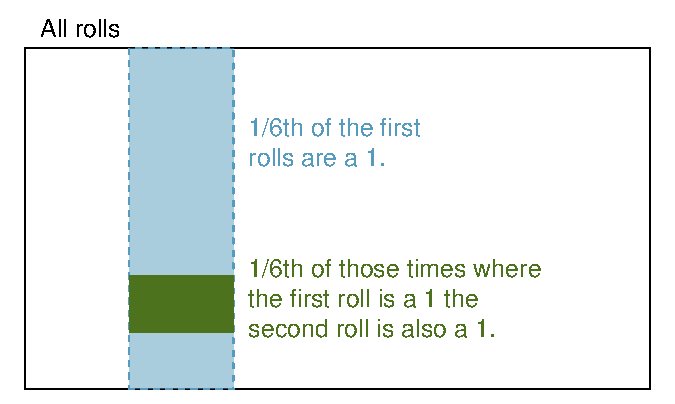
\includegraphics[width=0.6\textwidth]{ch_probability/figures/indepForRollingTwo1s/indepForRollingTwo1s}
\caption{$1/6$ of the time, the first roll is a \resp{1}. Then $1/6$ of \emph{those} times, the second roll will also be a \resp{1}.}
\label{indepForRollingTwo1s}
\end{figure}

\begin{ex}{What if there was also a blue die independent of the other two? What is the probability of rolling the three dice and getting all \resp{1}s?}\label{threeDice}
The same logic applies from Example~\ref{probOf2Ones}. If $1/36$ of the time the white and red dice are both \resp{1}, then $1/6$ of \emph{those} times the blue die will also be \resp{1}, so multiply:
{\begin{align*}
\P(white=\text{\small\resp{1} and } red=\text{\small\resp{1} and } blue=\text{\small\resp{1}})
	&= \P(white=\text{\small\resp{1}})\times \P(red=\text{\small\resp{1}})\times \P(blue=\text{\small\resp{1}}) \\
	&= (1/6)\times (1/6)\times (1/6)
	= 1/216
\end{align*}} \vspace{-7mm}
\end{ex}

Example~\ref{threeDice} illustrates what is called the \ask{Multiplication Rule} for independent processes \ask{or independent events}. 

\begin{defn}[Multiplication Rule for independent processes]
  \index{Multiplication Rule|textbf}%
  If $A$ and $B$ represent \ask{events} from two \ask{different} and
  \ask{independent} processes, then the probability that both $A$
  and $B$ occur can be calculated as the product of their
  separate probabilities:
  \begin{align*}
  \P(A \text{ and }B) = \P(A) \times  \P(B)
  \end{align*}
  Similarly, if there are $k$ events $A_1$, ..., $A_k$
  from $k$ independent processes, then the probability
  they all occur is
  \begin{align*}
  \P(A_1) \times  \P(A_2)\times  \cdots \times  \P(A_k)
  \end{align*}\vspace{-6mm}
\end{defn}

\begin{todo} \label{ex2Handedness}
About 9\% of people are left-handed. Suppose 2 people are selected at random from the U.S. population. Because the sample size of 2 is very small relative to the population, it is reasonable to assume these two people are independent. (a)~What is the probability that both are left-handed? (b)~What is the probability that both are right-handed?\footnotemark
\end{todo}
\footnotetext{(a) The probability the first person is left-handed is $0.09$, which is the same for the second person. We apply the Multiplication Rule for independent processes to determine the probability that both will be left-handed: $0.09\times 0.09 = 0.0081$.

(b) It is reasonable to assume the proportion of people who are ambidextrous (both right- and left-handed) is nearly 0, which results in $\P($right-handed$)=1-0.09=0.91$. Using the same reasoning as in part~(a), the probability that both will be right-handed is $0.91\times 0.91 = 0.8281$.}

\begin{todo}
\label{ex5Handedness}%
Suppose 5 people are selected at random.\footnotemark\vspace{-1.5mm}
\begin{enumerate}
\setlength{\itemsep}{0mm}
\item What is the probability that all are right-handed?
\item[(b)] What is the probability that all are left-handed?
\item[(c)] What is the probability that not all of the people are right-handed?
\end{enumerate}
\end{todo}
\footnotetext{(a)~The abbreviations \resp{RH} and \resp{LH} are used for right-handed and left-handed, respectively. Since each are independent, we apply the Multiplication Rule for independent processes:
\begin{align*}
\P(\text{all five are \resp{RH}})
&= \P(\text{first = \resp{RH}, second = \resp{RH}, ..., fifth = \resp{RH}}) \\
&= \P(\text{first = \resp{RH}})\times \P(\text{second = \resp{RH}})\times  \dots \times \P(\text{fifth = \resp{RH}}) \\
&= 0.91\times 0.91\times 0.91\times 0.91\times 0.91 = 0.624
\end{align*}

(b)~Using the same reasoning as in~(a), $0.09\times 0.09\times 0.09\times 0.09\times 0.09 = 0.0000059$

(c)~Use the complement, $\P($all five are \resp{RH}$)$, to answer this question:
\begin{align*}
\P(\text{not all \resp{RH}})
	= 1 - \P(\text{all \resp{RH}})
	= 1 - 0.624 = 0.376
\end{align*}}

Suppose the variables \var{handedness} and
\var{sex} are independent,
i.e. knowing someone's \var{sex} provides no useful
information about their \var{handedness} and vice-versa.
Then we can compute whether a randomly selected person is
right-handed and female\footnote{The actual proportion of
  the U.S. population that is \resp{female} is about 50\%,
  and so we use 0.5 for the probability of sampling a woman.
  However, this probability does differ in other countries.}
using the Multiplication Rule:
\begin{align*}
\P(\text{right-handed and female})
    &= \P(\text{right-handed}) \times  \P(\text{female}) \\
    &= 0.91 \times  0.50 = 0.455
\end{align*}


\begin{todo}
Three people are selected at random.\footnotemark \vspace{-1.5mm}
\begin{enumerate}
\setlength{\itemsep}{0mm}
\item What is the probability that the first person is male and right-handed?
\item[(b)] What is the probability that the first two people are male and right-handed?.
\item[(c)] What is the probability that the third person is female and left-handed?
\item[(d)] What is the probability that the first two people are male and right-handed and the third person is female and left-handed?
\end{enumerate}
\end{todo}
\footnotetext{Brief answers are provided. (a)~This can be written in probability notation as $\P($a randomly selected person is male and right-handed$)=0.455$. (b)~0.207. (c)~0.045. (d)~0.0093.}

Sometimes we wonder if one outcome provides useful information about another outcome. The question we are asking is, are the occurrences of the two events independent? We say that two events $A$ and $B$ are independent if they satisfy
$\P(A \text{ and }B) = \P(A) \times  \P(B)$.

\begin{ex}{If we shuffle up a deck of cards and draw one, is the event that the card is a heart independent of the event that the card is an ace?}
The probability the card is a heart is $1/4$ and the probability that it is an ace is $1/13$. The probability the card is the ace of hearts is $1/52$.
We check whether $\P(A \text{ and }B) = \P(A) \times  \P(B)$
is satisfied:
\begin{align*}
\P({\color{red}\heartsuit})\times \P(\text{ace}) = \frac{1}{4}\times \frac{1}{13} = \frac{1}{52} 
					= \P({\color{red}\heartsuit}\text{ and ace})
\end{align*}
Because the equation holds, the event that the card is a heart and the event that the card is an ace are independent events.
\end{ex}
\begin{quote}
\textit{%
    ``You know, the most amazing thing happened to me tonight. I was coming here, on the way to the lecture, and I came in through the parking lot. And you won't believe what happened. I saw a car with the license plate ARW 357. Can you imagine? Of all the millions of license plates in the state, what was the chance that I would see that particular one tonight? Amazing!''
}
\end{quote}
\end{document}
